\documentclass[titlepage,a4paper]{article}

\usepackage[a4paper,margin=2.5cm]{geometry}
\usepackage[colorlinks=true,linkcolor=black,urlcolor=blue,bookmarksopen=true]{hyperref}
\usepackage{bookmark}
\usepackage{fancyhdr}
\usepackage[spanish]{babel}
\usepackage[utf8]{inputenc}
\usepackage[T1]{fontenc}
\usepackage{graphicx}
\usepackage{float}
\usepackage{comment}
\usepackage[table]{xcolor}
\usepackage{array}
\usepackage{amsmath}


\pagestyle{fancy}
\fancyhf{}
\fancyhead[L]{T.P - Heller, Zaton}
\fancyhead[R]{Modelación Numérica - FIUBA}
\renewcommand{\headrulewidth}{0.4pt}
\fancyfoot[C]{\thepage}
\renewcommand{\footrulewidth}{0.4pt}

\begin{document}
\selectlanguage{spanish}

\begin{titlepage}
    \noindent
    \begin{minipage}{0.45\textwidth}
        \includegraphics[width=5cm]{logofiuba.jpg}
    \end{minipage}
    \hfill
    \begin{minipage}{0.45\textwidth}
    \end{minipage}

    \centering
    \vfill
    {\Huge \bfseries 
Análisis numérico de un sistema vibratorio lineal y no lineal \par}
    \vspace{1cm}
    {\Large [CB051] Modelación Numérica - Curso 02 Tarela \par}
    \vspace{0.05cm}
    Trabajo Práctico - Primer cuatrimestre de 2025
    \vspace{1cm}

    \noindent\textbf{Estudiantes:}
    
    \vspace{0.5cm}
    
    \centering
    \renewcommand{\arraystretch}{1.4}
    \rowcolors{2}{white}{gray!10}
    \begin{tabular}{|p{5cm}|p{3cm}|p{6cm}|}
        \rowcolor{black!80}
        \textcolor{white}{\textbf{Nombre}} & 
        \textcolor{white}{\textbf{Padrón}} & 
        \textcolor{white}{\textbf{Mail}} \\
        \hline
        Enrique José Heller & 111605 & eheller@fi.uba.ar \\
        \hline
        Martín Zaton Cardozo & 112188 & mzaton@fi.uba.ar \\
        \hline
    \end{tabular}

    \vfill
\end{titlepage}

\tableofcontents
\newpage

\section{Objetivos}

El presente trabajo tiene como objetivo analizar la aplicabilidad de métodos numéricos en la resolución de modelos matemáticos que describen sistemas físicos oscilatorios, específicamente el sistema \textbf{masa-resorte-amortiguador}. Se busca abordar tanto el caso lineal como el no lineal, con el fin de comprender las diferencias e implicancias de cada modelo. Por otro lado, se pretende contrastar los resultados obtenidos mediante simulación computacional con las soluciones analíticas disponibles, evaluando la precisión y estabilidad de los métodos numéricos implementados. Finalmente, se analizará el efecto del tamaño de paso sobre la calidad de las aproximaciones numéricas, haciendo uso de los conceptos teóricos estudiados en el curso.

\section{Introducción}

Se parte de entender al estudio de sistemas oscilatorios como fundamental en diversas ramas de la ingeniería, tal que permite comprender la respuesta de estructuras y componentes mecánicos ante perturbaciones. Se interpreta al modelo \textbf{masa-resorte-amortiguador} como una base para el análisis de estos fenómenos, permitiendo describir el movimiento oscilatorio de un cuerpo sometido a fuerzas restauradoras y disipativas. 

A continuación, se abordará la resolución analítica y numérica del sistema lineal, haciendo especial énfasis en la comparación entre el \textbf{Metodo de Euler Explícito} y el de \textbf{Runge-Kutta de orden 2}, para distintos coeficientes de amortiguamiento relativo. Luego se dará lugar a la incorporación de la no linealidad y se propondrá un analisis a partir del \textit{Oscilador de Duffing}.

\section{Análisis del sistema lineal (modelo base)}

En primer lugar, se propone la siguiente ecuación diferencial como el modelo matemático que representa nuestro caso de estudio:

\[
m\,x''(t) + c\,x'(t) + k\,x(t) = 0
\]

Donde:  
\begin{table}[H]
\centering
\begin{tabular}{cl}
$x(t)$: & Desplazamiento de la masa \\
$m$: & Masa del cuerpo \\
$c$: & Coeficiente de amortiguamiento \\
$k$: & Constante elástica del resorte \\
%$\alpha$: & Coeficiente de rigidez no lineal (Duffing) \\
$t$: & Tiempo \\
\end{tabular}
\end{table}

A partir de dichas magnitudes, se define al coeficiente de amortiguamiento relativo como:

\[
\zeta = \frac{c}{2\sqrt{km}}
\]

Dicho coeficiente, nos caracteriza a nuestro sistema de la siguiente manera:
\begin{table}[H]
\centering
\begin{tabular}{c c l}
$\zeta < 1$ & $\Rightarrow$ & Sistema subamortiguado \\
$\zeta = 1$ & $\Rightarrow$ & Sistema críticamente amortiguado \\
$\zeta > 1$ & $\Rightarrow$ & Sistema sobreamortiguado \\
\end{tabular}
\end{table}


Esta característica de amortiguamiento será uno de los criterios mediante los cuales se evaluarán los métodos númericos presentados a continuación.

\subsection{Método de Euler Explícito}

Para el desarrollo de este método, se parte de reescribir la EDO de orden 2 presentada, como un sistema de dos ecuaciones de primer orden. Para ello, se procede a definir las siguientes variables de estado $u(t)$ y $v(t)$:

\[
\begin{array}{rcl}
u(t) &=& x(t) \\
v(t) &=& {x'}(t)
\end{array}
\]

A partir de este cambio de variables y la EDO de orden 2 definida originalmente, es posible plantear el siguiente sistema de ecuaciones diferenciales de primer orden:

\[
\begin{cases}
u'(t) = v(t) \\
v'(t) = \dfrac{-c\,v(t) + k\,u(t)}{m}
\end{cases}
\]

La aplicación del método de Euler Explicito ímplica un proceso de discretización, tanto de la variable independiente \textit{t}, como las ecuaciones diferenciales ordinarias. 

Para \textit{t}, que es variable continua, la reescribimos como una serie de $n$ puntos que se encuentran a paso $h$ (no necesariamente constante pero que se define como tal por simplicidad de calculo)  esto significa que:

\[
t = n . h
\]

Para las EDOs de primer orden, se discretiza cada ecuación por separado, siendo a $u^n$  y $v^n$ las aproximaciones númericas de las funciones fuente para el instante $t_n$.

Para la primera ecuación, $u'(t) = v(t)$: Discretizamos la derivada $u'(t)$ en $t_n$ como:
\[
u'(t) \approx \dfrac{u^{n+1} - u^n}{h}
\]

Igualando esto a la aproximación de la función fuente y despejando $u^{n+1}$ se obtiene la fórmula de avance para esta ecuación:

\[
u^{n+1} = u^n + h \cdot v^n
\]

Haciendo lo propio para la segunda ecuación, se tiene que:

\[
v'(t) \approx \dfrac{v^{n+1} - v^n}{h} 
\]

\[
v^{n+1} = v^n + h \cdot \left(\dfrac{-c.v^n + k.u^n}{m}\right)
\]

Resultando así en el siguiente sistema de avance que nos permite realizar una aproximación a la solución de la EDO de segundo orden original:

\[
\begin{cases}
u^{n+1} = u^n + h \cdot v^n) \\
v^{n+1} = v^n + h \cdot \left(\dfrac{-c.v^n + k.u^n}{m}\right)
\end{cases}
\]

A partir de este sistema y la definición de las condiciones iniciales y constantes que nos definen los casos particulares a analizar, se define el algoritmo que permite realizar las aproximaciones pertinentes a este método que se retomará posteriormente.

\subsubsection{Análisis de precisión y estabilidad}

    Respecto a la precisión, se puede demostrar que el error de truncamiento en este método es de orden $\mathcal{O}(h)$. Esto hace que el método de Euler Explícito se clasifique como un método de orden 1, lo que implica que, al reducir el paso de discretización $h$ a la mitad, se espera que el error de truncamiento (y el error global, bajo ciertas condiciones) también se reduzca aproximadamente a la mitad. Lo propio se estudiará si ocurre empíricamente.

    Es esperable también en este método que haya \textbf{consistencia}, es decir, que cuando el paso \textit{h} tiende a 0, el error de truncamiento (que es el principal) también. Otro factor que resultará interesante de analizar empíricamente.

    Para el análisis de estabilidad del método, se procederá a utilizar el método de perturbaciones o \textit{método de Von Neumann}. Para ello, se introducirán pequeñas perturbaciones \(\delta u_n,\, \delta v_n\) en las variables para un instante $t_n$ y se analiza cómo estas perturbaciones se transforman en el instante siguiente $t_{n+1}$:
    
    \begin{align*}
        u_{n+1} + \delta u_{n+1} &= u_n + \delta u_n + h (v_n + \delta v_n), \\
        v_{n+1} + \delta v_{n+1} &= v_n + \delta v_n + h (-5 (v_n + \delta v_n) - 100 (u_n + \delta u_n)).
    \end{align*}

    Esto lo podemos ver como un sistema de ecuaciones que relaciona las perturbaciones en el paso $n+1$ con las perturbaciones en el paso $n$, restando las ecuaciones originales:

    \begin{align*}
        \delta u_{n+1} &= \delta u_n + h \cdot \delta v_n, \\
        \delta v_{n+1} & = -100\,h\,\delta u_n + (1 - 5h)\,\delta v_n
    \end{align*}

    De dicho sistema es posible definir la \textbf{matriz de amplificación} que describe cómo las perturbaciones se amplifican o decaen de un paso al siguiente:

    \[
    \begin{bmatrix}
    1 & h \\
    -100h & 1 - 5h
    \end{bmatrix}
    \]

    Para que el esquema numérico sea estable, las perturbaciones no deben crecer. Esto se traduce en la condición de que el radio espectral de la matriz de amplificación debe ser menor o igual a 1. Para este caso (haciéndonos valer de la herramienta \textit{WolframAlpha}, los autovalores resultan en:

    \[
        \lambda_1 = \frac{2 - 5h - 5i\sqrt{15}h}{2}, \quad \lambda_2 = \frac{2 - 5h + 5i\sqrt{15}h}{2}
    \]

    El hecho de que los autovalores sean complejos conjugados indica que la solución numérica corresponde a un comportamiento oscilatorio, lo cual resulta coherente para nuestro sistema. 

    Para que el sistema resulte estable (el radio espectral de la matriz sea menor o igual a 1), las cuentas correspondientes (también mediante \textit{WolframAlpha}) indican la siguiente condición:
    
    \[
    0 \leq h \leq \frac{1}{20} \approx 0.05
    \]
    
    Lo cual se verificará empíricamente. 


\subsection{Método de Runge-Kutta de orden 2}

Para este método, también se parte de reescribir la EDO de segundo orden como un sistema de dos ecuaciones de primer orden, utilizando las mismas variables de estado $u(t)$ y $v(t)$:

\[
\begin{cases}
u'(t) = v(t) \\
v'(t) = \dfrac{-c\,v(t) - k\,u(t)}{m}
\end{cases}
\]

El método de Runge-Kutta de orden 2 (RK2) permite obtener una mejor aproximación que el método de Euler, ya que utiliza información adicional del sistema en cada paso. Al igual que el método de Euler Explícito, implica el mismo proceso de discretización, del cual nos podemos valer.

El esquema predictor-corrector para este sistema es el siguiente:

\begin{itemize}
    \item \textbf{Paso predictor:}

    Se realiza una primera estimación de los valores en el instante $t^{n+1}$ utilizando las derivadas (evaluadas en las funciones fuente) en el instante actual $t^n$, de manera similar a Euler explícito:
     
    \begin{align*}
        u^*_{n+1} &= u_n + h \cdot v_n \\
        v^*_{n+1} &= v_n + h \cdot \left(\dfrac{-c\,v_n - k\,u_n}{m}\right)
    \end{align*}

    
    \item \textbf{Paso corrector:}

    Se corrigen las estimaciones obtenidas en el paso predictor, utilizando un promedio de las derivadas (evaluadas en las funciones fuente) en el instante $t^n$ y en el instante $t^{n+1}$ utilizando los valores predichos ($u^{n+1}$ y $v^{n+1}$):
    
    \begin{align*}
        u^{n+1} &= u^n + \frac{h}{2} (v^n + v^*^{n+1}) \\
        v^{n+1} &= v^n + \frac{h}{2} \left[ \dfrac{-c.v^n - k.u^n}{m} + \dfrac{-c.v^{*n+1} - k.u^{*n+1}}{m} \right]
    \end{align*}
\end{itemize}

De forma tal que $u^*_{n+1}$ y $v^*_{n+1}$ son los valores predichos en el paso predictor, y $u_{n+1}$ y $v_{n+1}$ son los valores corregidos que se utilizan para el siguiente paso.

Se parte de suponer que el método, al considerar el promedio de la pendiente inicial y la precalculada, mejora la precisión respecto de Euler, lo cual ínvita a estudiarse empíricamente.

A partir de este sistema y la definición de las condiciones iniciales y constantes que nos definen los casos particulares a analizar, se implementa el algoritmo de Runge-Kutta de orden 2 para obtener las aproximaciones numéricas correspondientes.

\subsubsection{Análisis de precisión y estabilidad}

En cuanto a la precisión de este método, de acuerdo a la teoría se espera que sea de orden O(2). Esto implicaría que el error de truncamiento sea proporcional a $h^2$ (despreciando términos de orden superior), lo que sugiere que al reducir el paso de discretización $h$ a la mitad, el error global (bajo ciertas condiciones) se espera que se reduzca aproximadamente a la cuarta parte. Otro elemento a verificar empíricamente.

Respecto a la estabilidad, cabe destacar que este esquema resulta explícito, ya que los valores en el paso $n+1$ se calculan directamente a partir de valores ya conocidos en el paso $n$ y los valores predichos en el paso $n+1$, por lo que es condicionalmente estable al igual que Euler Explicito.

Dada la complejidad que implica calcular el radio espectral de la matriz de amplificación para este caso, se opta por verificar empíricamente el rango de estabilidad para el paso $h$, a partir de observar el comportamiento en los valores propuestos. 

\subsection{Resultados empíricos}

A partir del marco analítico previamente presentado, se ofrece a continuación un análisis empírico y comparativo entre los métodos presentados. Para ello, pasamos a establecer cuál será el marco común para realizar dicha comparativa, con el fin de que los contrastes entre los resultados se deban unicamente a la variación de amortiguación del sistema, lo que resultar de interés estudiar para este trabajo.

\subsubsection{Condiciones Iniciales}

Dentro del rango propuesto por la cátedra, se optó por establecer las siguientes constantes comunes a todos los casos de prueba:

\begin{itemize}
    \item $u_0 = 10^{-2} {m}$
    \item $v_0 = 1 \frac{m}{s}$
    \item Pasos de integración: $h \in \{0.1s,\ 0.05s,\ 0.025s\} $
    \item Tiempos finales: $t_{\text{final}} \in \{0.5s,\ 2s,\ 5s,\ 10s\}$
\end{itemize}



\subsubsection{Caso subamortiguado (\(\zeta < 1\))}

Para el estudio de este caso, se tomaron los siguientes valores:

\begin{itemize}
    \item \( m = 1kg \)
    \item \( c = 5 \frac{Ns}{m} \)
    \item \( k = 100 \frac{N}{m} \)
\end{itemize}

Lo que significa un $\zeta = 0.25$.



Se procedió entonces a obtener una solución analítica del modelo mediante la herramienta \textit{WolframAlpha} y se obtuvo la siguiente solución:

\[
x(t) = e^{-\frac{5t}{2}} \left(
   0{,}01\,\cos\left(\tfrac{5\sqrt{15}}{2}t\right)
   + 0{,}105862\,\sin\left(\tfrac{5\sqrt{15}}{2}t\right)
\right).
\]

Dicha solución resultó de utilidad para medir los errores de los modelos propuestos.

A continuación, se muestra una comparativa entre la solución óptima y las aproximaciones calculadas para los distintos $h_s$, para ambos modelos presentados:


\begin{figure}[H]
  \centering
  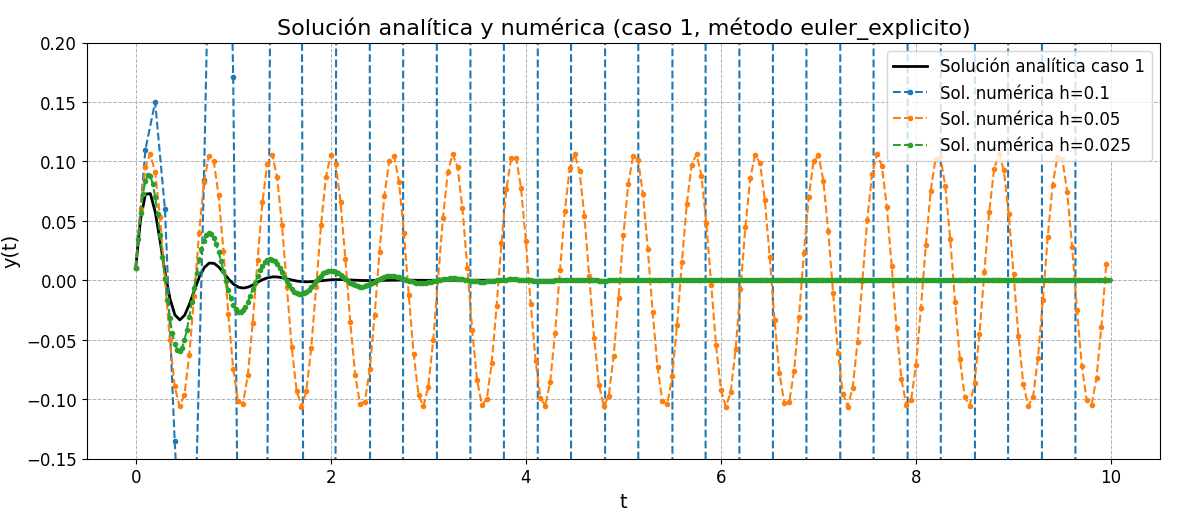
\includegraphics[width=\textwidth]{resultados/comparacion_analitica_aproximada/euler_explicito/z=0.25/caso 1.png}
  \label{fig:euler_subamortiguado}
\end{figure}

\begin{figure}[H]
  \centering
  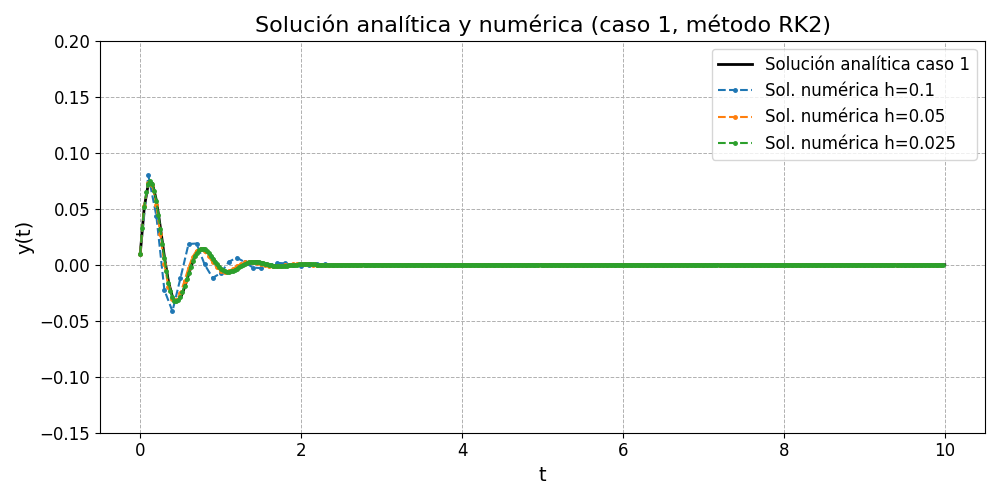
\includegraphics[width=\textwidth]{resultados/comparacion_analitica_aproximada/RK2/z=0.25/caso 1_2.png}
  \label{fig:euler_subamortiguado}
\end{figure}

Saraza saraza Saraza saraza Saraza saraza Saraza saraza Saraza saraza Saraza saraza Saraza saraza Saraza saraza Saraza saraza Saraza saraza.Saraza saraza Saraza saraza Saraza saraza Saraza saraza Saraza saraza Saraza saraza Saraza saraza Saraza saraza Saraza saraza Saraza saraza Saraza saraza Saraza saraza Saraza saraza Saraza saraza Saraza saraza Saraza saraza Saraza saraza Saraza saraza Saraza saraza Saraza saraza Saraza saraza Saraza saraza Saraza saraza Saraza saraza. Saraza saraza Saraza saraza Saraza saraza Saraza saraza Saraza saraza Saraza saraza Saraza saraza Saraza saraza Saraza saraza Saraza saraza.Saraza saraza Saraza saraza Saraza saraza Saraza saraza Saraza saraza Saraza saraza Saraza saraza Saraza saraza Saraza saraza Saraza saraza Saraza saraza Saraza saraza Saraza saraza Saraza saraza Saraza saraza Saraza saraza Saraza saraza Saraza saraza Saraza saraza Saraza saraza Saraza saraza Saraza saraza Saraza saraza Saraza saraza Saraza saraza.


% --- Caso críticamente amortiguado ---

\subsubsection{Caso críticamente amortiguado ($\zeta = 1$)}

Para el estudio de este caso, se tomaron los siguientes valores:

\begin{itemize}
    \item $m = 0.1\,\text{kg}$
    \item $c = 0.55\,\frac{\text{Ns}}{\text{m}}$
    \item $k = 0.625\,\frac{\text{N}}{\text{m}}$
\end{itemize}

Lo que significa un $\zeta = 1$.

Se procedió entonces a obtener una solución analítica del modelo mediante la herramienta \textit{WolframAlpha} y se obtuvo la siguiente solución:

\[
x(t) = -0.443438\,\exp\left(-3.89564\,t\right) + 0.453438\,\exp\left(-1.60436\,t\right)
\]

Dicha solución resultó de utilidad para medir los errores de los modelos propuestos.

A continuación, se muestra una comparativa entre la solución óptima y las aproximaciones calculadas para los distintos $h_s$, para ambos modelos presentados:

\begin{figure}[H]
  \centering
  \includegraphics[width=\textwidth]{resultados/comparacion_analitica_aproximada/euler_explicito/z=1/caso_2.png}
  \caption{Comparación entre la solución analítica y las aproximaciones numéricas (Euler Explícito) para el caso críticamente amortiguado.}
\end{figure}

\begin{figure}[H]
  \centering
  \includegraphics[width=\textwidth]{resultados/comparacion_analitica_aproximada/RK2/z=1/caso_2.png}
  \caption{Comparación entre la solución analítica y las aproximaciones numéricas (Runge-Kutta 2) para el caso críticamente amortiguado.}
\end{figure}

% --- Caso sobreamortiguado ---

\subsubsection{Caso sobreamortiguado ($\zeta > 1$)}

Para el estudio de este caso, se tomaron los siguientes valores:

\begin{itemize}
    \item $m = 10\,\text{kg}$
    \item $c = 10\,\frac{\text{Ns}}{\text{m}}$
    \item $k = 0.5\,\frac{\text{N}}{\text{m}}$
\end{itemize}

Lo que significa un $\zeta = 3.16$.

Se procedió entonces a obtener una solución analítica del modelo mediante la herramienta \textit{WolframAlpha} y se obtuvo la siguiente solución:

\[
x(t) = -1.11862\,\exp\left(-0.947214\,t\right) + 1.12862\,\exp\left(-0.0527864\,t\right)
\]

Dicha solución resultó de utilidad para medir los errores de los modelos propuestos.

A continuación, se muestra una comparativa entre la solución óptima y las aproximaciones calculadas para los distintos $h_s$, para ambos modelos presentados:

\begin{figure}[H]
  \centering
  \includegraphics[width=\textwidth]{resultados/comparacion_analitica_aproximada/euler_explicito/z=3.16/caso_3.png}
  \caption{Comparación entre la solución analítica y las aproximaciones numéricas (Euler Explícito) para el caso sobreamortiguado.}
\end{figure}

\begin{figure}[H]
  \centering
  \includegraphics[width=\textwidth]{resultados/comparacion_analitica_aproximada/RK2/z=3.16/caso_3.png}
  \caption{Comparación entre la solución analítica y las aproximaciones numéricas (Runge-Kutta 2) para el caso sobreamortiguado.}
\end{figure}


\section{Incorporación de no linealidad y análisis del oscilador de Duffing}

Saraza saraza Saraza saraza Saraza saraza Saraza saraza Saraza saraza Saraza saraza Saraza saraza Saraza saraza Saraza saraza Saraza saraza.Saraza saraza Saraza saraza Saraza saraza Saraza saraza Saraza saraza Saraza saraza Saraza saraza Saraza saraza Saraza saraza Saraza saraza Saraza saraza Saraza saraza Saraza saraza Saraza saraza Saraza saraza Saraza saraza Saraza saraza Saraza saraza Saraza saraza Saraza saraza Saraza saraza Saraza saraza Saraza saraza Saraza saraza Saraza saraza. Saraza saraza Saraza saraza Saraza saraza Saraza saraza Saraza saraza Saraza saraza Saraza saraza Saraza saraza Saraza saraza Saraza saraza.Saraza saraza Saraza saraza Saraza saraza Saraza saraza Saraza saraza Saraza saraza Saraza saraza Saraza saraza Saraza saraza Saraza saraza Saraza saraza Saraza saraza Saraza saraza Saraza saraza Saraza saraza Saraza saraza Saraza saraza Saraza saraza Saraza saraza Saraza saraza Saraza saraza Saraza saraza Saraza saraza Saraza saraza Saraza saraza.


\section{Conclusiones}

% Aquí puedes redactar las conclusiones

\section{Anexos}
\subsection{Código implementado}
% Aquí va el código fuente en verbatim o listings.

\subsection{Corridas numéricas}
% Aquí pueden ir gráficos adicionales, tablas o referencias a datos.

\end{document}
